\chapter[Cơ sở lý thuyết và nghiên cứu liên quan]{Cơ sở lý thuyết và\\nghiên cứu liên quan}
\label{chap:background}

Chương này hệ thống hóa bốn khối kiến thức nền tảng làm tiền đề lý thuyết cho toàn bộ thiết kế mô hình ở Chương~\ref{chap:method}: (1) đặc điểm bệnh học lâm sàng của MCI và ý nghĩa của dữ liệu theo dõi dọc; (2) khung phân tích sống còn cùng cơ chế xử lý chuỗi thời gian có khoảng cách không đều; (3) đặc tính biểu diễn của ba nguồn dữ liệu đa phương thức đầu vào; và (4) nguyên lý hợp nhất đa phương thức thông qua phân rã tensor CP kết hợp kết nối phần dư có cổng điều tiết. Cuối chương, tôi tổng quan các hướng tiếp cận liên quan trong y văn và phân tích các khoảng trống nghiên cứu then chốt mà khóa luận tập trung giải quyết.

\section{MCI, dữ liệu dọc và bài toán tiên lượng}
Năm 2018, Viện Lão khoa Quốc gia và Hiệp hội Alzheimer Hoa Kỳ (NIA-AA) đã đề xuất khung nghiên cứu cập nhật, định nghĩa bệnh Alzheimer (AD) dựa trên các dấu ấn sinh học thực thể thay vì chỉ chờ đợi các triệu chứng lâm sàng bộc lộ ra bên ngoài \cite{jack2018niaaa}. Theo đó, hệ thống phân loại AT(N) phân biệt ba nhóm dấu ấn sinh học: sự lắng đọng mảng amyloid-$\beta$ (A), protein tau bệnh lý (T) cùng tổn thương hoặc thoái hóa tế bào thần kinh (N). Đáng chú ý, các biến đổi bệnh lý này có thể âm thầm xuất hiện từ nhiều năm trước khi người bệnh biểu hiện triệu chứng sa sút trí tuệ rõ rệt; trong đó A và T mang tính đặc hiệu cho căn bệnh Alzheimer, còn (N) phản ánh mức độ tổn thương thần kinh tiến triển có thể bắt nguồn từ nhiều cơ chế khác nhau \cite{jack2018niaaa}.

Về mặt lâm sàng, suy giảm nhận thức nhẹ (Mild Cognitive Impairment -- MCI) được định vị ở ranh giới chuyển tiếp giữa lão hóa sinh lý bình thường và sa sút trí tuệ thực thụ: người bệnh đã suy giảm trí nhớ hoặc khả năng tư duy ở một số khía cạnh song vẫn có khả năng tự chủ trong phần lớn các sinh hoạt thường nhật. Tổng kết từ các nghiên cứu dịch tễ và theo dõi dọc dài hạn của Petersen và cộng sự chỉ ra rằng các cá thể mắc MCI không đi theo một quỹ đạo bệnh lý duy nhất: một tỷ lệ đáng kể sẽ nhanh chóng chuyển biến thành sa sút trí tuệ, trong khi các nhóm khác có thể duy trì trạng thái ổn định lâu dài hoặc thậm chí hồi phục về mức nhận thức bình thường \cite{petersen2018mci}. Chính vì vậy, mục tiêu cốt lõi của bài toán tiên lượng là phát hiện sớm những người có nguy cơ suy giảm nhanh nhằm tối ưu hóa chiến lược can thiệp và ưu tiên nguồn lực theo dõi lâm sàng.

Để ghi nhận tường minh tiến trình biến đổi sinh học đó, Sáng kiến Hình ảnh Thần kinh Bệnh Alzheimer (ADNI) đã thu thập dữ liệu ảnh MRI quét lặp lại theo thời gian từ nhiều trung tâm nghiên cứu lâm sàng \cite{jack2008adnimri,weiner2015impact}. So với việc chỉ khảo sát một lần chụp cắt ngang đơn lẻ, việc phân tích chuỗi chụp lặp lại của cùng một bệnh nhân cho phép mô hình định lượng chính xác tốc độ biến đổi vi mô và vĩ mô của cấu trúc não bộ — tiêu biểu như tốc độ teo vùng hồi hải mã trong phương pháp sử dụng cặp MRI dọc của Dong và cộng sự \cite{dong2021deepatrophy}.

\section{Phân tích sống còn và mô hình thời gian}
\subsection{Biến cố, kiểm duyệt và mô hình rủi ro tỷ lệ Cox}
Trong các nghiên cứu lâm sàng theo dõi dọc dài hạn, câu hỏi thực tiễn không chỉ dừng lại ở việc ``ai sẽ suy giảm nhận thức'' mà mang tính thời điểm sâu sắc hơn: ``ai có nguy cơ tiến triển \emph{sớm hơn}''. Giả sử một người tham gia được theo dõi suốt 2 năm rồi dừng nghiên cứu khi trạng thái nhận thức vẫn hoàn toàn ổn định: ta không thể biết chắc ở năm thứ 3 họ có tiến triển thành sa sút trí tuệ hay không, nhưng hoàn toàn khẳng định được rằng trong suốt 2 năm đầu tiên biến cố chưa hề xảy ra. Hiện tượng thông tin bị gián đoạn này được gọi là \emph{kiểm duyệt phải} (right-censoring) \cite{kaplan1958nonparametric,cox1972regression}. Nếu ép bài toán về dạng phân loại nhị phân Có/Không truyền thống, ta buộc phải gán nhãn sai lệch hoặc loại bỏ hoàn toàn các đối tượng kiểm duyệt này, dẫn đến nguy cơ sai lệch chọn mẫu nghiêm trọng. Khung phân tích sống còn giải quyết triệt để hạn chế trên bằng cách mô hình hóa đồng thời hai biến số ngẫu nhiên cho mỗi cá thể $i$: thời gian theo dõi $t_i$ và chỉ báo biến cố $\delta_i$ ($\delta_i=1$ nếu ghi nhận biến cố tại $t_i$, và $\delta_i=0$ nếu đối tượng bị kiểm duyệt phải tại lần khám cuối cùng). Hình~\ref{fig:concept-survival} minh họa sinh động hai kịch bản lâm sàng này.

\begin{figure}[H]
\centering
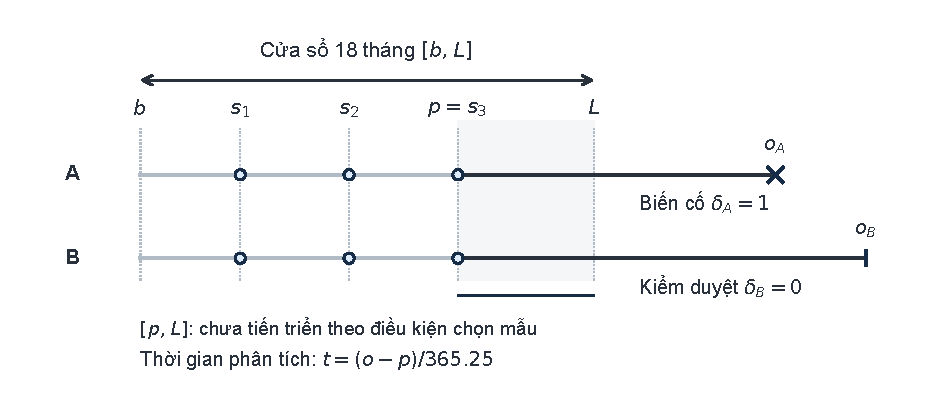
\includegraphics[width=\textwidth]{image/concept-survival.pdf}
\caption{Khái niệm biến cố và kiểm duyệt phải trong phân tích sống còn}
\label{fig:concept-survival}
\end{figure}

Mô hình rủi ro tỷ lệ Cox \cite{cox1972regression} mô tả tốc độ xảy ra biến cố tức thời (hàm nguy cơ) $h_i(t)$ của cá thể $i$ tại thời điểm $t$ thông qua tích của hai thành phần:
\begin{equation}
 h_i(t)=h_0(t)\exp(\eta_i).
 \label{eq:cox-hazard}
\end{equation}
Trong đó, $h_0(t)$ là \emph{hàm nguy cơ nền} chung của toàn bộ quần thể theo thời gian, còn $\eta_i = f_\theta(x_i)$ đại diện cho \emph{điểm log-nguy cơ} của cá thể $i$, được ước lượng từ đặc trưng đầu vào $x_i$ qua mạng nơ-ron sâu với tham số $\theta$ (tương tự như nguyên lý của mô hình DeepSurv \cite{katzman2018deepsurv}). Ưu điểm vượt trội của mô hình Cox nằm ở chỗ: tỷ số nguy cơ (Hazard Ratio) giữa hai cá thể $i$ và $j$ bằng $\exp(\eta_i - \eta_j)$, hoàn toàn độc lập với thời gian $t$. Điều này đồng nghĩa với việc cá thể nào sở hữu điểm log-nguy cơ $\eta$ cao hơn thì sẽ có xác suất xảy ra biến cố cao hơn ở bất kỳ thời điểm nào trong suốt quá trình theo dõi.

Nhờ tính chất độc lập thời gian đó, trong quá trình huấn luyện mạng nơ-ron, ta không cần phải ước lượng hàm nguy cơ nền $h_0(t)$ phức tạp mà chỉ cần cực tiểu hóa hàm đối log-hợp lý riêng phần Cox (Cox partial log-likelihood) \cite{cox1972regression,katzman2018deepsurv}:
\begin{equation}
 \mathcal L_{\rm Cox}=-\sum_{i:\delta_i=1}\left[\eta_i-\log\sum_{j\in\mathcal R(t_i)}\exp(\eta_j)\right],
 \label{eq:cox-loss}
\end{equation}
trong đó $\mathcal R(t_i)=\{j:t_j\geq t_i\}$ là \emph{tập nguy cơ} gồm tất cả những người vẫn đang được theo dõi và chưa gặp biến cố ngay trước thời điểm $t_i$. Về mặt trực giác, hàm mất mát này buộc mô hình phải gán chỉ số nguy cơ $\eta_i$ của người vừa ghi nhận biến cố cao hơn chỉ số $\eta_j$ của những người vẫn đang an toàn trong cùng tập nguy cơ; đồng thời, các đối tượng bị kiểm duyệt phải vẫn đóng góp tích cực vào mẫu số chuẩn hóa $\mathcal R(t_i)$ cho tới thời điểm họ rời khỏi nghiên cứu. Trong trường hợp xuất hiện các biến cố xảy ra trùng thời điểm, tôi áp dụng xấp xỉ Breslow để các ca trùng mốc có thể dùng chung tập nguy cơ một cách nhất quán \cite{breslow1974covariance}. Để đánh giá năng lực xếp hạng của mô hình, thước đo chuẩn mực được áp dụng là chỉ số đồng thuận Harrell's C-index — đại diện cho tỷ lệ các cặp đối tượng có thể so sánh được mà trong đó người gặp biến cố sớm hơn được mô hình gán điểm nguy cơ cao hơn một cách chính xác \cite{harrell1996multivariable}.

Trong phân tích dữ liệu dọc, một khái niệm quan trọng có liên quan là \emph{dự báo tại mốc xác định} (landmarking): tại một mốc thời gian ấn định trước, mô hình chỉ sử dụng những thông tin đã thu thập trước mốc đó để tiến hành dự báo cho những người còn lại trong nhóm nguy cơ \cite{vanhouwelingen2007dynamic}. Quy trình xác định cửa sổ quan sát và mốc chọn mẫu cụ thể của khóa luận được trình bày chi tiết ở Chương~\ref{chap:method}.

\subsection{Mạng nơ-ron thời gian T-LSTM và cơ chế chú ý}
\label{sec:background-temporal}
Mạng bộ nhớ dài ngắn hạn (LSTM) xử lý chuỗi thời gian hiệu quả bằng cách duy trì và cập nhật trạng thái bộ nhớ qua từng bước tuần tự \cite{hochreiter1997lstm}. Tuy nhiên, kiến trúc LSTM truyền thống ngầm định rằng khoảng cách thời gian giữa các bước liên tiếp luôn bằng nhau. Trong thực tế hồ sơ bệnh án y tế, khoảng cách giữa hai lần thăm khám liên tiếp biến thiên rất lớn: có thể là 3 tháng ở bệnh nhân này nhưng lại lên tới 12 tháng ở bệnh nhân khác. Rõ ràng, thông tin thu thập từ 12 tháng trước thường suy giảm độ liên quan đến tình trạng hiện tại so với dữ liệu vừa đo đạc cách đây 3 tháng \cite{baytas2017patient}.

Kiến trúc mạng T-LSTM (Time-Aware LSTM) do Baytas và cộng sự đề xuất \cite{baytas2017patient} đã giải quyết trọn vẹn hạn chế này bằng cách đưa trực tiếp khoảng thời gian thực tế $\Delta t$ giữa hai lần khám vào phương trình cập nhật bộ nhớ: trạng thái bộ nhớ trước đó $c_{t-1}$ được phân rã thành thành phần dài hạn (được bảo tồn nguyên vẹn) và thành phần ngắn hạn (được điều tiết suy giảm phi tuyến theo hàm số của $\Delta t$) trước khi tổng hợp cùng thông tin mới của lần khám hiện tại.

Sau khi T-LSTM tạo ra chuỗi trạng thái ẩn $h_t$ tương ứng với từng thời điểm khám, thay vì chỉ lấy thụ động trạng thái cuối cùng, mô hình áp dụng cơ chế chú ý cộng (additive attention) để tổng hợp thích ứng toàn bộ các lần khám với trọng số học trực tiếp từ dữ liệu. Ý tưởng tổng hợp có trọng số bắt nguồn từ Bahdanau và cộng sự \cite{bahdanau2015attention}; trong khóa luận, tôi triển khai cấu trúc chấm điểm thông qua một vectơ ngữ cảnh học được $\bm v$ theo Yang và cộng sự \cite{yang2016hierarchical}:
\begin{equation}
 e_t=\bm v^\top\tanh(W_hh_t+b_h),\qquad
 \alpha_t=\frac{\exp(e_t)}{\sum_k\exp(e_k)},\qquad
 z=\sum_t\alpha_th_t.
 \label{eq:additive-attention}
\end{equation}
Trong đó, hệ số $\alpha_t \in (0,1)$ phản ánh mức độ đóng góp thông tin của lần khám thứ $t$, còn $z$ là vectơ biểu diễn tổng hợp giàu ý nghĩa cho toàn bộ tiến trình lịch sử thăm khám của người bệnh. Hình~\ref{fig:concept-longitudinal} minh họa nguyên lý phối hợp nhịp nhàng giữa T-LSTM và cơ chế attention trên chuỗi ba lần khám.

\begin{figure}[H]
\centering
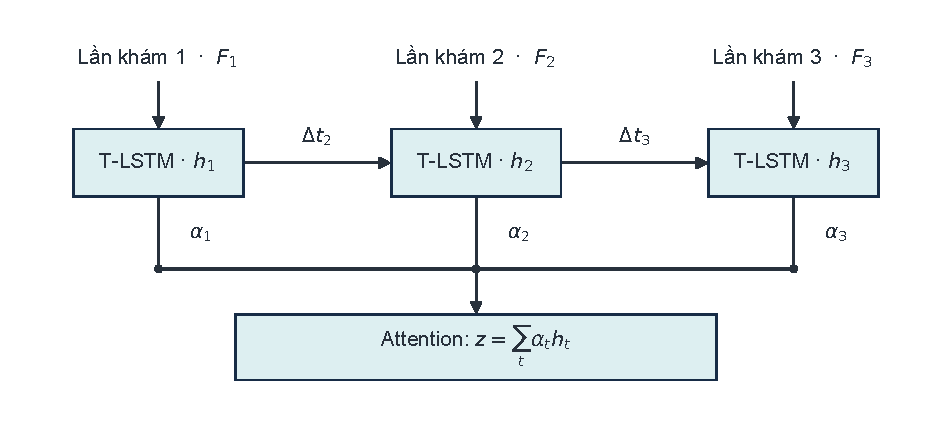
\includegraphics[width=\textwidth]{image/concept-longitudinal.pdf}
\caption{Nguyên lý tổng hợp chuỗi dữ liệu dọc có khoảng cách không đều bằng T-LSTM và attention}
\label{fig:concept-longitudinal}
\end{figure}

\section{Ba nguồn thông tin và đặc trưng biểu diễn}
Khóa luận tích hợp đồng thời ba nguồn dữ liệu chuẩn mực và phổ biến trong nghiên cứu bệnh Alzheimer: ảnh MRI cấu trúc 3D, đặc trưng radiomics toàn não và các thang điểm đánh giá lâm sàng. Bảng~\ref{tab:background-inputs} và Hình~\ref{fig:concept-sources} tóm tắt bản chất thông tin cùng các lưu ý kỹ thuật riêng biệt của từng phương thức.

\begin{table}[H]
\centering\small
\caption[Ba nguồn thông tin trong bài toán]{Bản chất thông tin và điểm cần lưu ý của ba nguồn dữ liệu.}
\label{tab:background-inputs}
\begin{tabularx}{\linewidth}{@{}L{2.5cm}Y Y@{}}
\toprule
\textbf{Nguồn} & \textbf{Thông tin chính} & \textbf{Điểm cần lưu ý} \\
\midrule
MRI cấu trúc 3D & Hình thái giải phẫu não; trích đặc trưng tự động bằng CNN 3D & Cần đồng nhất tư thế, kích thước lưới và thang cường độ mà không làm méo hình học \\
Radiomics & Chỉ số định lượng về hình dạng, phân bố độ sáng và kết cấu mô ảnh & Giá trị đặc trưng kết cấu phụ thuộc cách rời rạc hóa mức xám \cite{zwanenburg2020ibsi} \\
Lâm sàng & Điểm kiểm tra nhận thức (MMSE) và chức năng sinh hoạt (CDR) & Liên quan trực tiếp tiêu chí biến cố; cần tách bạch đầu vào và kết cục \\
\bottomrule
\end{tabularx}
\end{table}

\begin{figure}[H]
\centering
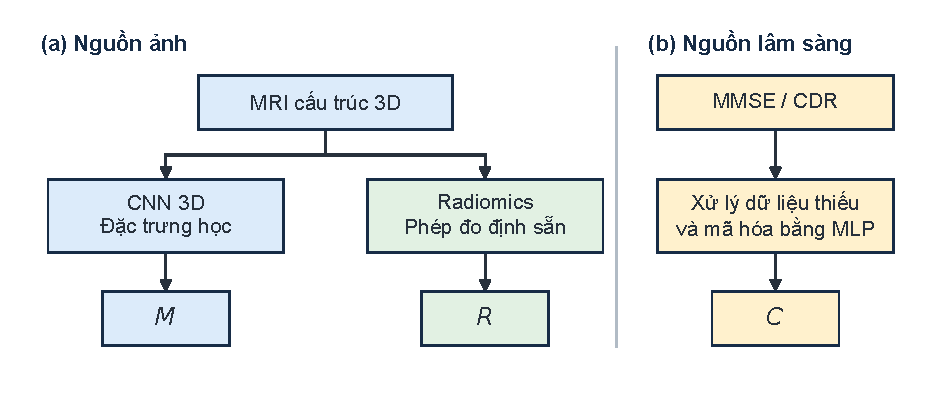
\includegraphics[width=\textwidth]{image/concept-sources.pdf}
\caption{Mối quan hệ và nguồn gốc của ba luồng biểu diễn dữ liệu tại mỗi lần khám}
\label{fig:concept-sources}
\end{figure}

Cụ thể hơn, mỗi nguồn thông tin đảm nhận một vai trò biểu diễn chuyên biệt:
\begin{enumerate}
\item \emph{Ảnh MRI cấu trúc 3D}: phản ánh trực quan hình thái giải phẫu não tại thời điểm quét \cite{jack2008adnimri}. Trong lĩnh vực học sâu y khoa, các kiến trúc tích chập phần dư 3D như ResNet \cite{he2016deep}, đặc biệt khi được khởi tạo từ bộ trọng số tiền huấn luyện trên khối dữ liệu ảnh y khoa 3D đa dạng như MedicalNet \cite{chen2019med3d}, thường được ưu tiên sử dụng để học biểu diễn trực tiếp từ thể tích toàn não — thay vì chỉ trích xuất cục bộ tại vùng hồi hải mã như một số công trình trước đây \cite{li2019hippocampal}.
\item \emph{Đặc trưng radiomics}: đại diện cho các chỉ số định lượng toán học được định nghĩa tường minh nhằm mô tả hình học không gian, phân bố thống kê cường độ sáng và hoa văn kết cấu của vùng mô não (chẳng hạn mức độ tương phản từ ma trận đồng xuất mức xám GLCM). Các định nghĩa này đã được cộng đồng IBSI chuẩn hóa chặt chẽ \cite{zwanenburg2020ibsi} và tích hợp hoàn chỉnh trong thư viện PyRadiomics \cite{vangriethuysen2017computational}. Do các đặc trưng radiomics thường có số lượng lớn và tương quan nội bộ cao, kỹ thuật phân tích thành phần chính (PCA) \cite{jolliffe2016pca} là công cụ thích hợp để nén chiều hiệu quả trước khi đưa vào mạng nơ-ron.
\item \emph{Dữ liệu lâm sàng}: thang điểm MMSE \cite{folstein1975mmse} phản ánh chức năng nhận thức tổng quát, trong khi thang CDR \cite{morris1993cdr} đánh giá toàn diện cả nhận thức lẫn khả năng tự chủ sinh hoạt thường ngày. Các chỉ số thu thập trong giai đoạn quan sát đầu vào cung cấp tín hiệu bổ trợ trực tiếp về hiện trạng của người bệnh, hoàn toàn tách biệt với các lần đo sau mốc chọn mẫu dùng để xác định biến cố kết cục.
\end{enumerate}

\section{Hợp nhất đa phương thức và tham số hóa tương tác}
\label{sec:background-fusion}
Sau khi mỗi nguồn dữ liệu được ánh xạ thành một vectơ biểu diễn đặc trưng, bài toán then chốt tiếp theo là hợp nhất chúng thành một không gian biểu diễn chung \cite{baltrusaitis2019multimodal}. Phương thức tiếp cận trực quan và phổ biến nhất là \emph{ghép nối} (concatenation): xếp các vectơ thành phần nối tiếp nhau để hình thành một vectơ dài hơn. Ưu điểm của phép ghép nối là không làm phát sinh thêm tham số tại bước kết hợp; tuy nhiên, hạn chế cố hữu của nó là không tạo ra được các tương tác chéo bậc hai trực tiếp giữa các nguồn dữ liệu, do đó toàn bộ mối liên hệ phi tuyến phức tạp hoàn toàn bị phó mặc cho các lớp ẩn phía sau tự học.

Trái ngược với điều đó, \emph{phép tích ngoài} (outer product) tiến hành nhân từng tọa độ của nguồn thứ nhất với từng tọa độ của nguồn thứ hai, qua đó kiến tạo tường minh mọi cặp tương tác song tuyến bậc hai \cite{zadeh2017tensor}. Hình~\ref{fig:concept-fusion} minh họa trực quan sự khác biệt cơ bản này trên hai vectơ hai chiều: phép ghép nối chỉ sinh ra một vectơ 4 phần tử độc lập tuyến tính, trong khi phép tích ngoài tạo nên một ma trận $2\times2$ chứa trọn vẹn cả bốn tích chéo $x_i y_j$.

\begin{figure}[H]
\centering
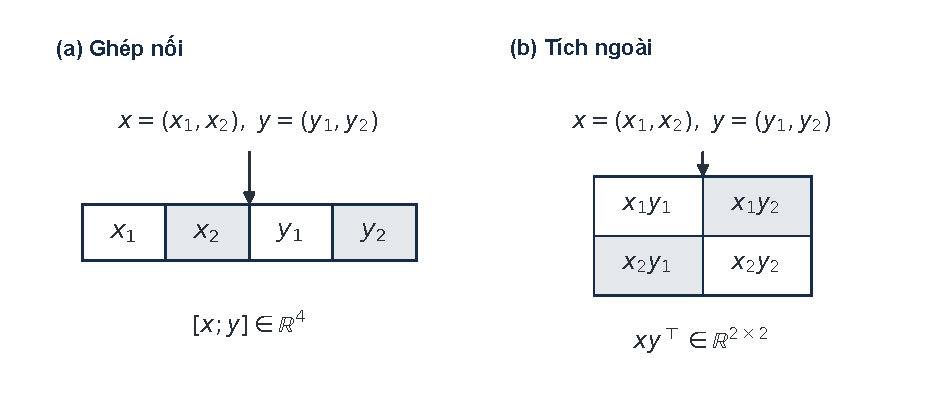
\includegraphics[width=\textwidth]{image/concept-fusion.pdf}
\caption{So sánh phép ghép nối và phép tích ngoài trên ví dụ hai chiều}
\label{fig:concept-fusion}
\end{figure}

\subsection{Từ tích ngoài đến phân rã tensor CP hạng thấp}
Rào cản lớn nhất khi ứng dụng phép tích ngoài nằm ở hiện tượng bùng nổ tham số tính toán. Xét hai vectơ đặc trưng bất kỳ $x\in\mathbb R^{d_x}$ và $y\in\mathbb R^{d_y}$. Nếu trải phẳng ma trận tích ngoài $xy^\top \in \mathbb R^{d_x\times d_y}$ rồi chiếu qua một lớp tuyến tính thông thường sang không gian đầu ra $d_o$ chiều, mỗi tọa độ đầu ra $h_k$ ($k=1,\dots,d_o$) sẽ là một tổ hợp có trọng số của mọi tích chéo:
\begin{equation}
 h_k=\sum_{i=1}^{d_x}\sum_{j=1}^{d_y}\mathcal W_{kij}x_i y_j+b_k,
 \label{eq:full-bilinear}
\end{equation}
trong đó $\mathcal W\in\mathbb R^{d_o\times d_x\times d_y}$ đóng vai trò là một tensor trọng số bậc ba. Khi đó, số lượng tham số cần tối ưu hóa lên tới $d_o d_x d_y$ (chưa bao gồm độ chệch $b$). Xét trường hợp kích thước thực tế trong khóa luận ($d_x=32$, $d_y=32$ và $d_o=128$), chỉ riêng một lớp tương tác đơn lẻ này đã ngốn tới $32 \times 32 \times 128 = 131\,072$ trọng số — một con số quá lớn so với tập huấn luyện khiêm tốn gồm vài trăm bệnh nhân, khiến mô hình đối mặt với nguy cơ quá khớp nghiêm trọng \cite{liu2018lowrank}.

Để tháo gỡ nút thắt bùng nổ tham số đó mà vẫn giữ được năng lực nắm bắt tương tác song tuyến, kỹ thuật \emph{phân rã tensor Canonical Polyadic (CP)} \cite{carroll1970candecomp,kolda2009tensor} xấp xỉ tensor trọng số bậc ba $\mathcal W$ thông qua tổng của $Q$ thành phần hạng một, với $Q$ là một hằng số nhỏ gọi là \emph{hạng phân rã}:
\begin{equation}
 \mathcal W_{kij}\approx\sum_{q=1}^Q O_{kq}A_{iq}B_{jq}.
 \label{eq:cp-concept-math}
\end{equation}
Khi thay thế biểu thức~(\ref{eq:cp-concept-math}) vào phương trình~(\ref{eq:full-bilinear}) và hoán đổi thứ tự lấy tổng, phép chiếu tích ngoài ba chiều cồng kềnh được rút gọn thành chuỗi ba phép toán cực kỳ tinh gọn:
\begin{equation}
 h=O\bigl[(A^\top x)\odot(B^\top y)\bigr]+b,
 \label{eq:cp-hadamard}
\end{equation}
trong đó $A\in\mathbb R^{d_x\times Q}$, $B\in\mathbb R^{d_y\times Q}$ và $O\in\mathbb R^{d_o\times Q}$ là ba ma trận nhân tử hạng thấp được tối ưu trực tiếp bằng giải thuật lan truyền ngược, còn $\odot$ là phép nhân từng phần tử (Hadamard). Thay vì phải nhân chéo toàn bộ các cặp tọa độ trong không gian ban đầu rồi mới nén lại, cơ chế phân rã CP thực hiện chiếu trước $x$ và $y$ về không gian tiềm ẩn $Q$ chiều, tiến hành nhân từng phần tử trong không gian hạng thấp này rồi mới chiếu tuyến tính ra không gian đích $d_o$ chiều (Hình~\ref{fig:cp-intro}). Trở lại ví dụ kích thước $d_x=32, d_y=32, d_o=128$: nếu chọn hạng $Q=8$, số lượng trọng số cần học giảm ngoạn mục từ $131\,072$ xuống chỉ còn $Q(d_x + d_y + d_o) = 8 \times (32+32+128) = 1\,536$ (tương đương mức giảm gần 99\%). Ý tưởng tham số hóa hạng thấp này cũng chính là nguyên lý cốt lõi của các mô hình hợp nhất đa phương thức tiên tiến như LMF \cite{liu2018lowrank} và MUTAN \cite{benyounes2017mutan}.

\begin{figure}[H]
\centering
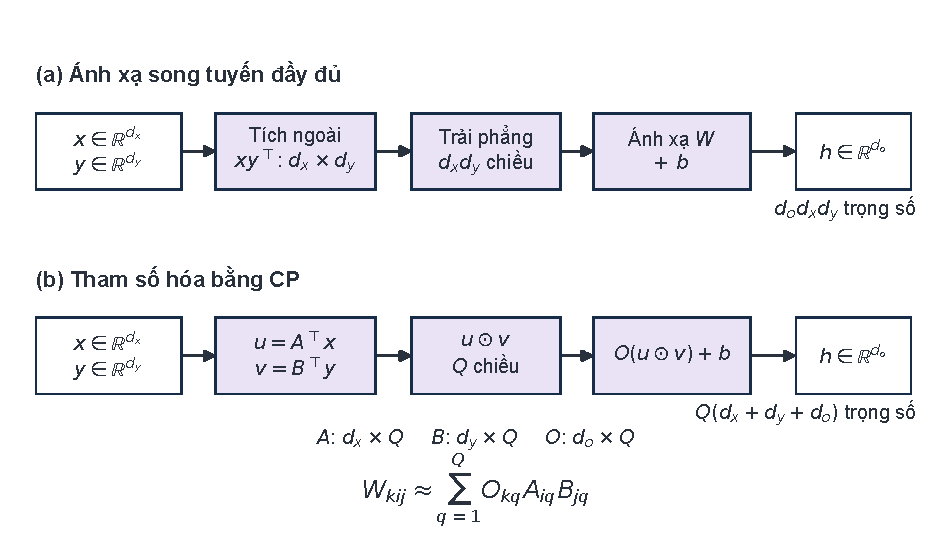
\includegraphics[width=\textwidth]{image/cp-concept-general.pdf}
\caption{So sánh ánh xạ song tuyến đầy đủ và tham số hóa CP hạng thấp}
\label{fig:cp-intro}
\end{figure}

\subsection{Nguyên lý kết nối phần dư có cổng điều tiết}
Sau khi thu được biểu diễn tương tác song tuyến giữa hai nguồn, nếu thay thế hoàn toàn đặc trưng gốc bằng đặc trưng tương tác thì mô hình sẽ đứng trước nguy cơ đánh mất các tín hiệu đặc thù của từng phương thức, đặc biệt khi một trong hai nguồn gặp nhiễu đo đạc. Nhằm khắc phục điểm yếu này, một nguyên lý hiệu quả trong hợp nhất đa phương thức là \emph{kết nối phần dư có cổng điều tiết} (gated residual fusion): duy trì đường truyền trực tiếp của biểu diễn gốc và chỉ cộng bổ sung thành phần tương tác sau khi đã qua một cổng kiểm soát thích ứng phụ thuộc vào chính dữ liệu đầu vào.

Nguyên lý này đã chứng minh tính hiệu quả ở nhiều miền bài toán khác nhau; hai công trình gần đây trên arXiv trong xử lý video đa phương thức minh họa cho các biến thể tiêu biểu:
\begin{enumerate}
\item \emph{Text Residual Fusion} của Ryumina và cộng sự (2026) \cite{ryumina2026residual}: sử dụng biểu diễn văn bản làm luồng thông tin trung tâm, trong khi các luồng âm thanh, khuôn mặt và bối cảnh đóng góp các thành phần phần dư thông qua các cổng phụ thuộc đầu vào trước khi tiến hành chuẩn hóa (Hình~\ref{fig:literature-gates}(a)).
\item \emph{DyFADet+} của Liu và cộng sự (2026) \cite{liu2026motion}: sử dụng luồng ảnh RGB làm trục truyền dẫn chính, còn đặc trưng chuyển động khung xương được đưa qua cổng kiểm soát và nhân với hệ số cố định $\alpha=0.5$ trước khi cộng dồn phần dư (Hình~\ref{fig:literature-gates}(b)).
\end{enumerate}

\begin{figure}[H]
\centering
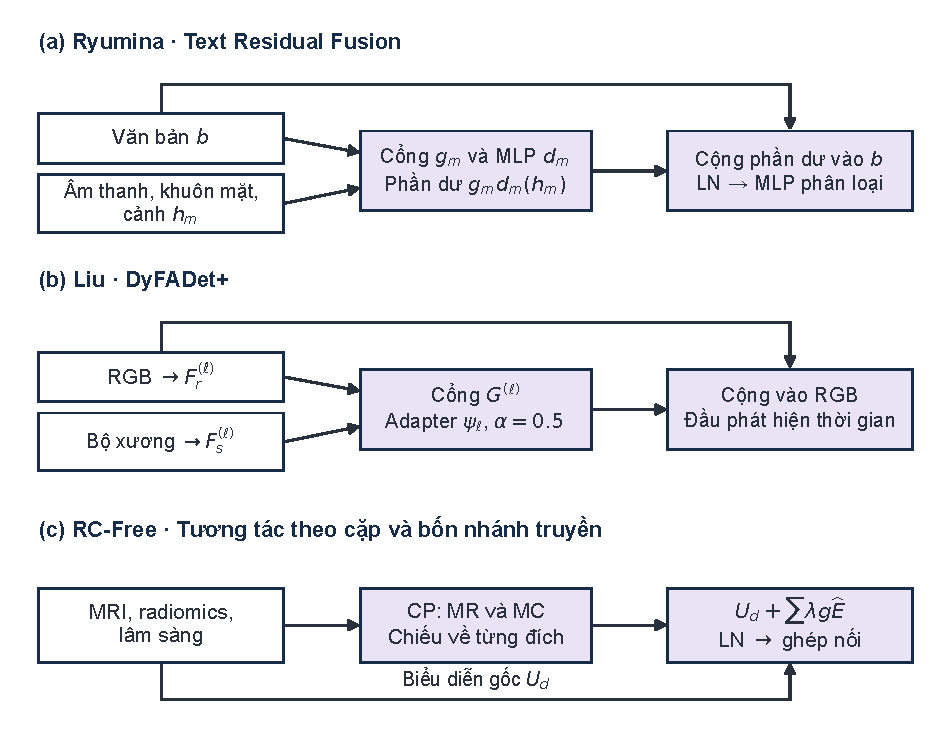
\includegraphics[width=\textwidth]{image/literature-gates.pdf}
\caption[Các cơ chế kết nối phần dư có cổng]{Minh họa nguyên lý kết nối phần dư có cổng do tác giả tổng hợp: (a) theo mô hình của Ryumina và cộng sự \cite{ryumina2026residual}, (b) theo mô hình của Liu và cộng sự \cite{liu2026motion}, và (c) sơ đồ áp dụng phần dư có cổng cho từng nguồn trong kiến trúc của khóa luận.}
\label{fig:literature-gates}
\end{figure}

Khác với hai mô hình trên vốn chỉ neo phần dư vào một nguồn chủ đạo duy nhất, trong kiến trúc đề xuất của khóa luận, mỗi nguồn dữ liệu đều bảo tồn đường truyền biểu diễn riêng biệt và tiếp nhận các phần dư tương tác thông qua các cổng điều tiết độc lập kết hợp hệ số tỷ lệ học được (minh họa tổng quan ở Hình~\ref{fig:literature-gates}(c)). Các công thức toán học và thiết kế chi tiết của cơ chế này được trình bày hoàn chỉnh ở Mục~\ref{sec:gated-routing} thuộc Chương~\ref{chap:method}.

\section{Nghiên cứu liên quan và khoảng trống nghiên cứu}
\label{sec:related-work}
Trong những năm gần đây, nhiều phương pháp học máy và học sâu tiên tiến đã được nghiên cứu nhằm giải quyết bài toán tiên lượng tiến triển từ MCI sang sa sút trí tuệ. Bảng~\ref{tab:related} hệ thống hóa bốn hướng tiếp cận tiêu biểu trong y văn và chỉ rõ mối liên hệ kế thừa của khóa luận.

\begin{table}[H]
\centering\small
\renewcommand{\arraystretch}{1.02}
\caption[Tổng hợp nghiên cứu liên quan]{Các hướng nghiên cứu chính, công trình tiêu biểu và điểm khóa luận kế thừa.}
\label{tab:related}
\begin{tabularx}{\linewidth}{@{}L{2.8cm}Y Y@{}}
\toprule
\textbf{Hướng tiếp cận} & \textbf{Công trình và cách làm} & \textbf{Liên hệ với khóa luận} \\
\midrule
MRI đơn thời điểm & Li: ảnh hồi hải mã; Nakagawa: thể tích chất xám và mạng sống còn \cite{li2019hippocampal,nakagawa2020survival} & Khung biểu diễn ảnh MRI và bài toán sống còn \\
Dữ liệu dọc & Li và Fan: MRI đầu và nhận thức dọc \cite{li2019early}; Ding: chuỗi nhận thức và MRI \cite{ding2023progression}; Dong: biến đổi từ cặp MRI \cite{dong2021deepatrophy} & Khai thác thông tin thay đổi theo thời gian cho tiên lượng \\
Radiomics và lâm sàng & Tang và cộng sự: LASSO--Cox kết hợp radiomics, lâm sàng và xét nghiệm \cite{tang2021individualized} & Động lực kiểm chứng giá trị bổ sung của radiomics và lâm sàng \\
MRI dọc học sâu & Aghajanian và cộng sự: CNN--PCA--T-LSTM, attention và hàm mất mát Cox \cite{aghajanian2025longitudinal} & Quy trình tham chiếu, định nghĩa biến cố và phân tầng nguy cơ \\
\bottomrule
\end{tabularx}
\end{table}

Trong số các công trình kể trên, nghiên cứu của Aghajanian và cộng sự \cite{aghajanian2025longitudinal} đóng vai trò là điểm xuất phát tham chiếu trực tiếp nhất. Nhóm tác giả đã lựa chọn 228 đối tượng mắc MCI từ bộ dữ liệu ADNI có tối thiểu ba lần chụp MRI T1 trong 18 tháng đầu, sử dụng mạng CNN để trích xuất đặc trưng từng ảnh, nén chiều bằng PCA trên tập huấn luyện (giữ lại 99\% phương sai giải thích), rồi huấn luyện mô hình T-LSTM (có khảo sát cơ chế attention) với hàm mất mát Cox. Đáng chú ý, khi thử nghiệm bổ sung thêm đặc trưng radiomics chất xám vào mô hình T-LSTM có attention, năng lực phân biệt C-index của mô hình lại giảm nhẹ thay vì tăng, dẫn đến việc mô hình cuối cùng chỉ duy trì duy nhất đặc trưng trích từ ảnh MRI \cite{aghajanian2025longitudinal}.

\subsection{Khoảng trống nghiên cứu}
\label{sec:research-gaps}
Cần nhấn mạnh rằng, kết luận về vai trò mờ nhạt của radiomics trong công trình của Aghajanian và cộng sự vốn gắn liền với phương thức ghép nối đặc trưng đơn giản và quy trình xử lý hai bước phân tách độc lập. Kết quả đó chưa thể khẳng định liệu việc mô hình hóa tường minh các tương tác chéo song tuyến giữa MRI với radiomics và lâm sàng trong một kiến trúc học sâu đầu-cuối có thể khai phá tiềm năng của các nguồn dữ liệu này hay không. Xuất phát từ khoảng trống nghiên cứu then chốt đó, tôi đề xuất kiểm chứng hai định hướng thiết kế mới trong một quy trình huấn luyện đầu-cuối thống nhất:
\begin{enumerate}[itemsep=0.1em,topsep=0.2em]
\item \emph{Tham số hóa tương tác cặp bằng phân rã tensor CP}: thay thế lớp song tuyến đầy đủ bằng cấu trúc CP hạng $Q$ nhằm vừa nắm bắt các mối liên hệ chéo bậc hai, vừa kiểm soát chặt chẽ số lượng tham số cần tối ưu.
\item \emph{Lược bỏ tương tác trực tiếp dư thừa (RC-Free)}: duy trì đầy đủ cả ba nguồn dữ liệu đầu vào song chỉ kích hoạt hai cặp tương tác xoay quanh ảnh MRI (MR và MC) và chủ động lược bỏ cặp RC, sau đó đối chiếu khách quan với toàn bộ các tổ hợp cặp khác ở Chương~\ref{chap:results}.
\end{enumerate}
